\section{Auswertung}

\subsection{Überprüfung der Bragg-Bedingung}

Bei einem Kristallwinkel von $\theta_{\text{K}} = 14{\textdegree}$ wurde der Winkel $\theta_{\text{GM}}$ vom Geiger-Müllerzählrohr variiert und die Zählrate gemessen.
Die Werte sind in Tabelle \ref{tab:ogemessdaten1} angegeben und lassen sich nun in ein Diagramm \ref{fig:plot1} mit Winkelabhängigkeit einzeichnen.
\begin{figure}[h]
  \centering
  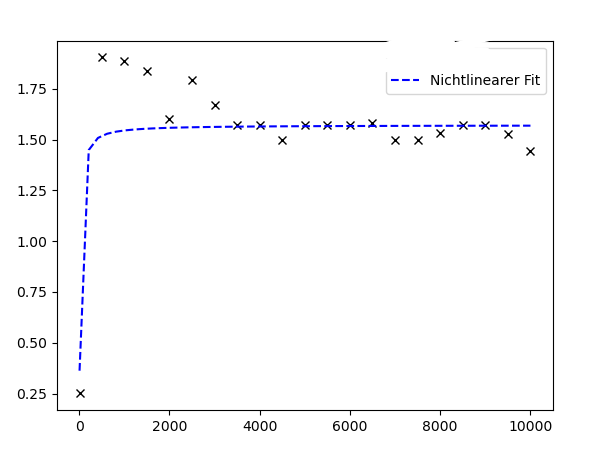
\includegraphics[width=\textwidth]{build/plot1.pdf}
  \caption{Zählratendiagramm mit Winkelabhängigkeit.}
  \label{fig:plot1}
\end{figure}
Der Winkel mit der höchsten Zählrate lässt sich am Diagramm \ref{fig:plot1} und an den Messwerten \ref{tab:ogemessdaten1} als
\begin{equation}
\theta_{\text{max}} = 28{,}2{\textdegree}
\end{equation}
feststellen.
Die theoretische Lage des Maximums, also der Sollwert hat einen Winkel von $\theta_{\text{soll}} = 28{\textdegree}$. Somit ergibt sich folgende Abweichung vom Sollwert.
\begin{equation}
\increment \theta = \theta_{\text{max}} - \theta_{\text{soll}} = 0{,}2{\textdegree}
\end{equation}

\subsection{Analyse eines Emissionsspektrums einer Kupfer-Röntgenröhre}

Das Emissionsspektrum wurde mit einer Integrationszeit von $\increment t = \SI{10}{\second}$ in jeweils $\increment \theta_{\text{K}} = 0{,}1\textdegree$ Abständen gemessen.
Die Zählraten lässen sich nun zusammen mit einem Po

\begin{figure}[h]
  \centering
  \includegraphics[width=\textwidth]{build/plot2.pdf}
  \caption{Röntgenspektrum einer Kupfer-Röntgenröhre.}
  \label{fig:plot2}
\end{figure}